
\chapter{Erstellung der Software}
\label{cha:erstellung}
In diesen Abschnitt beschreiben wir den Erstellungsprozess der
Software. Dazu beschreiben wir erst die Struktur des Projektes, den
Aufbau des Buildsystems für den Client und schließlich den Erstellungsprozess für
Client und Server.
% und am Ende schließlich
%die Benutzung von Client und Server.


\section{Aufbau des Projektbaums}
\label{sec:aufbau_projektbaum}
Der aus dem SVN ausgecheckte Projektbaum  ist wie folgt aufgebaut:\\
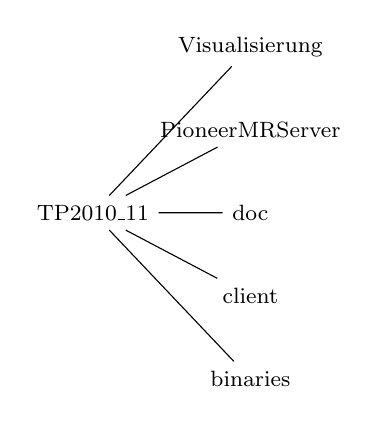
\begin{tikzpicture}
%\tikz 
[font=\footnotesize,
       grow=right, level 1/.style={sibling distance=3em},
                   level 2/.style={sibling distance=1em}, level distance=2cm]
  \node {TP2010\_11} % root
     child { node {binaries}}
     child {node {client}}
   child{node {doc} }
   child{node {PioneerMRServer}
     }
  child{node {Visualisierung}
    }; %
\end{tikzpicture}
Da beim Client es nötig war, diverse Libaries des Institutes für
Robotik und Prozessinformatik (IRP) der technischen Universität
Braunschweig sowie den Sonar-Partikelfilter und die Ballerkennung zu
integrieren, wurde dazu eine besondere Buildumgebung auf Basis von
CMake geschaffen. Sie
wird im Abschnitt \ref{cha:integr-best-proj} ab Seite
\pageref{cha:integr-best-proj} beschrieben. Einen ersten Überblick
über die Struktur des Ordners ,,client'' gibt folgende Baumübersicht:\\
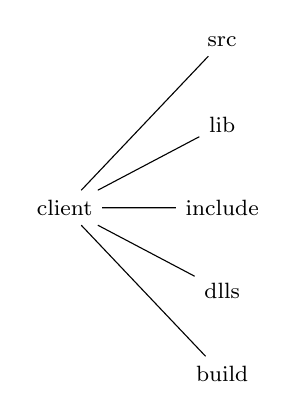
\begin{tikzpicture}
%\tikz 
[font=\footnotesize,
       grow=right, level 1/.style={sibling distance=3em},
                   level 2/.style={sibling distance=1em}, level distance=2cm]
  \node {client} % root
     child { node {build}}
     child {node {dlls}}
   child{node {include} }
   child{node {lib}
     }
  child{node {src}
    }; %
\end{tikzpicture}
Der Ordner ,,build'' enthält die durch CMake generierten VisualStudio
Projekte und fertig gebauten ausführbaren Dateien und DLLs. Die Ordner
,,dlls'' und ,,lib'' enthalten zur Erzeugung und Ausführung der
Projekte nötige externe *dll und *lib Dateien. In den Ordnern
,,include'' und ,,src'' sind schließlich die Quelltexte und Header der
verwendeten Libaries sowie unseres Clients ,,p3dxSteuerung''
enthalten. \\\\
Die Notwendigkeit einer gesondereten Buildinfrastruktur war beim
Server (PioneerMRServer) nicht 
gegeben, da dieser nicht von den Institutsbibliotheken
abhängt. Entsprecht reichte es dort, ein normales VisualStudio Projekt
zu erstellen. 

%%% Local Variables: 
%%% mode: latex
%%% TeX-master: "template"
%%% End: 

\section{Integration bestehender Projekte in ein neues Buildsystem für den
Client}
\label{cha:integr-best-proj}
\subsection{Warum ein neues Buildsystem?}
Die Ballerkennung und der Sonarpartikelfilter hängen von vielen
Altprojekten
ab. Das Beispiel für die Steuerung der Pioneer 3-DX hing zudem von der ARIA
Bibliothek\footnote{http://robots.mobilerobots.com/wiki/ARIA} ab. Bei den
Altprojekten fanden sich auch zum Teil fest kodierte Pfade. Da auch die
Konvertierung der Solutions in das VS 2010 Format meistens fehlschlug und
auch
ARIA nicht mit der mitgelieferten Solution unter VS 2010 gebaut werden
konnte,
haben wir uns für den Client für den Einsatz eines neuen Buildsystems
entschlossen. Aufgrund der Einfacheit der Beschreibung der Buildvorgänge
für
die einzelnen zu integrierenden Projekte und dem Hinzufügen neuer
Unterprojekte, sowie der Möglichkeit, von einem konkreten Buildsystem
abhängig
zu sein sowie existierender Erfahrungen mit dem System, fiel die Wahl auf
CMake\footnote{http://www.cmake.org/}. Bei CMake handelt es sich um ein
open-source Metabuildsystem. Es erzeugt Build-Vorschriften für andere
Buildsysteme (u.a. GNU make, nmake, msbuild). Somit wäre es bei Bedarf auch
Möglich gewesen, auf eine andere Visual Studio Version umzusteigen ohne
die Solutions zu konvertieren oder neu zu erstellen.

\subsection{Integration der Projekte}
Zuerst wurde eine passende Ordnerstrukur angelegt: include für
Header-Dateien,
src für die cpp-Dateien der einzelnen Projekt, bin für eventuell zum Linken
 benötigte
Kompillate, deren Quellen nicht in den Build-Prozess integrierbar waren und
build als Zielordner für erzeugte Buildfiles.

Als nächstes wurde für das Projekt im Ordner des Clients eine
CMakeLists.txt-Datei angelegt:

\begin{lstlisting}[language={},captionpos=b,caption={CMakeLists.txt für das Buildsystem des Clients}]
cmake_minimum_required (VERSION 2.6)
project (TP_WS_2010)

include_directories (include)
include_directories (include/ControlExample)
include_directories (include/erob/)
include_directories (include/Balldetection)
include_directories (include/p3dxSteuerung)
include_directories (include/StochasticLib)
include_directories (include/PioneerMRClient)
include_directories (include/Aria)
include_directories (include/OccupancyGridMap)
include_directories (include/irpVideo/DirectShow)
link_directories (${TP_WS_2010_BINARY_DIR})
link_directories (${TP_WS_2010_SOURCE_DIR}/lib/)
add_subdirectory (src)
\end{lstlisting}

Diese definiert den Namen des Projektes (wichtig
für Referenzen auf z.b. das Stammverzeichnis des Projektes oder das
Buildverzeichnis, da die entprechenden Variablennamen mit dem Projektnamen
+ \_
als Präfix versehen werden. Zudem wurden die include-Verzeichnisse und zum
Linken relevante Verzeichnisse festgelegt. Danach wurde das src-Verzeichnis
 als
Projektunterordner hinzugefügt. Dadurch werden die Anweisungen in der
CMakeLists.txt des Unterordners auch ausgeführt. Dies ermöglicht es, für
die
einzelnen Unterprojekte jeweils eine eigene kleine CMakeLists.txt zu
verwenden.

Die CMakeLists.txt bindet nun alle Sourceordner der Unterprojekte ein:

\begin{lstlisting}[language={},captionpos=b,caption={CMakeLists.txt für den Sourceordner}]
%\begin{lstlisting}
cmake_minimum_required (VERSION 2.6)

add_subdirectory (irpUtils)
add_subdirectory (irpMath)
add_subdirectory (irpImage)
add_subdirectory (irpVideo)
add_subdirectory (irpFeatureExtraction)
add_subdirectory (alglib)
add_subdirectory (DistanceMap)
add_subdirectory (irpCamera)
add_subdirectory (irpV3d)
add_subdirectory (StochasticLib)
add_subdirectory (Visualization)
add_subdirectory (CamCalib)
add_subdirectory (Balldetection)
add_subdirectory (mathtest)
add_subdirectory (SonarParticleFilter)
add_subdirectory (PioneerMRClient)
add_subdirectory (OccupancyGridMap)
add_subdirectory (Balldetection_Test)
add_subdirectory (Aria)
add_subdirectory (p3dxSteuerung)
add_subdirectory (p3dxSteuerung_threaded)
add_subdirectory (calibrate)
#add_subdirectory (ControlExample)
add_subdirectory (utils)
add_subdirectory (kinect)
add_subdirectory (networkTest)
\end{lstlisting}

Bei den Unterprojekten gibt es zwei Arten: Bibliotheken und Anwendungen.

Die CMakeList.txt einer Bibliothek sieht wie folgt aus:
\begin{lstlisting}[language={},captionpos=b,caption={CMakeLists.txt einer Bibliothek am
    Beispiel irpCamera}]
%\begin{lstlisting}
cmake_minimum_required (VERSION 2.6)

file(GLOB src "*.cpp")
file(GLOB includes "../../include/irpCamera/*.h")

add_library (irpCamera ${src} ${includes})
\end{lstlisting}

Die CMakeList.txt einer Anwendung sieht so aus:
\begin{lstlisting}[language={},captionpos=b,caption={CMakeLists.txt des Clients}]
cmake_minimum_required (VERSION 2.6)

file(GLOB src "*.cpp")
file(GLOB includes "../../include/p3dxSteuerung/*.h")
add_executable (p3dxSteuerung_threaded ${src} ${includes})
target_link_libraries (p3dxSteuerung_threaded irpUtils MINPACK fftw rfftw
DirectShow irpFeatureExtraction irpMath  alglib irpImage irpCamera irpVideo
 irpV3d glew CamCalib Visualization StochasticLib OccupancyGridMap
SonarParticleFilter ws2_32 winmm advapi32 Aria DistanceMap Balldetection)

\end{lstlisting}

Zuerst werden alle cpp-Dateien zur Variablen src hinzugfügt, danach die
Includes zur Variablen include. Je nachdem, ob es sich um eine Bibliothek
oder
Anwendung handelt, wird diese mit add\_library(name dateien) oder
add\_executable(name dateien) hinzugefügt. Die Include-Dateien müssen dabei
aber eigentlich nicht explizit hinzugefügt werden, dies geschieht nur,
damit
sie auch in einer VS Solution in der Dateiliste auftauchen. Bei Anwendungen
können nun mit target\_link\_libraries(exename libraries) noch die zu
linkenden
Bibliotheken angegeben werden.

Es gab ein paar Probleme bei der Integration: zum einen mussten zuerst die
Abhängigkeiten zwischen den Unterprojekten ermittelt werden, dies geschah
mit
Hilfe der originalen VS Solutions sowie durch Ausprobieren. Zum anderen gab
 es
manchmal Dateien, die zwar in den Quellen lagen, jedoch in nicht in den
Solutions auftauchten. Diese konnten den Buildprozess stören und mussten
daher
entfernt werden TODO: Beispiel raussuchen, wenn noch überhaupt möglich.
Außerdem waren an ein paar Stellen kleinere Änderungen am Quellcode nötig,
um
ihn mit MSVC 2010 oder der Struktur unseres include-Ordners kompatibel zu
machen.

\subsection{Hinzufügen eines neuen Unterprojektes}
\label{sec:hinz-eines-neuen-unterprojektes}
Das Hinzufügen eines neuen Unterprojektes ist relativ einfach.
Zuerst wird ein Unterverzeichnis für das Projekt im include-Ordner und
eines im
src-Ordner angelegt. Dann kopiert man die includes in den neuen Unterordner
 im
include-Ordner. Dabei ist darauf zu achten, dass die Pfade in
\#include-Direktiven relative zum include-Ordner sein sollten. Danach
kopiert
man die cpp-Dateien in den neuen Unterordner im src-Verzeichnis.

Danach erstellt man in diesem Ordner eine CMakeLists.txt ähnlich wie oben,
jenachdem ob ex sich um eine Anwendung oder Bibliothek handelt. Man fügt
zuerst
die cpp-Dateien und Includes hinzu, fügt dann mit add\_library oder
add\_executable Buildtargets hinzu und gibt eventuell noch zu linkende
Bibliotheken bei Anwendungen an mit target\_link\_libraries.

%%% Local Variables: 
%%% mode: latex
%%% TeX-master: "template"
%%% End: 



\section{Erstellung von Client und Server mit Visual Studio  2010}
Da der Client mit Hilfe des im vorherigenen Abschnitts auf CMake
basierenden Buildystems erzeugt wird, sind hier mehr Schritte als beim
Server notwendig:
\begin{enumerate}
	\item CMake für Windows (Version min. 2.6) herunterladen und installieren
  \footnote{http://www.cmake.org/}
	\item CMake GUI starten
	\item Unter "Where is the source code" den Pfad des Client-Verzeichnisses
 eintragen und unter "Where to build the binaries" den Pfad zu dem
Verzeichnis, wo die Solution für den Client erstellt werden soll
	\item Auf "Configure" klicken, ,,Visual Studio 2010'' und ,,Use default
native compilers'' auswählen, dann auf Finish klicken. Auf das Ende des
Einrichtens warten.
	\item Auf "Generate" klicken.
	\item Im ausgewählten Zielverzeichnis befindet sich nun eine
          Visual Studio 2010
Solution (TP\_WS\_2010.sln). 
\item Außerdem befindet sich im Unterordner ,,PioneerMRServer'' im
Projektbaum eine Solution für den
Server (PioneerMRServer.sln). Beide Solutions können ganz normal mit 
Visual Studio 2010 geöffnet und gebaut werden (F7 oder STRG-Alt-F7).
\end{enumerate}

%%% Local Variables: 
%%% mode: latex
%%% TeX-master: "template"
%%% End: 

\chapter{Nutzung der Software}
\label{cha:nutzung}
\section{Client}
\label{sec:client-1}

\subsection{Kalibrierung der Balldetection}
\label{sec:kalibr-der-balld}
Die Ballerkennung muss zunächst kalibriert werden, da ansonsten keine
brauchbaren Ergebnisse erzielt werden können. Dies ist deshalb nötig,
da die Ausrichtung der auf dem Roboter montierten Webcam
entscheidenden Einfluss auf die von der Ballerkennung ermittelten
Werte hat. Zur VisualStudio Solution ,,TP2010/11'' gehört auch ein
Unterprojekt calib. Nach Erstellung der ausführbaren Datei calib.exe
ist diese an folgende Stelle des Projektbaums zu kopieren:
\verb|\client\src\calibrate\| \\ 
Für die folgenden Schritte werden dann ein Schachbrett sowie ein
Maßband oder Ähnliches benötigt. 
Danach geht man folgendermaßen vor:
\begin{itemize}
\item Man stellt das Schachbrett und den Roboter in einen Abstand von
  ca 1 Meter voneinander entfernt so auf, dass die Kamera auf die
  Mitte des Schachbrettes zeigt. 
% TODO: bild einfügen
\item Danach misst man mit dem Maßband die Entfernung zwischen Roboter
  und Schachbrett, sowie den Abstand vom Schachbrett zum Boden (im
  Normallfall 25 cm). Die
  beiden Enden der Entfernungstrecke zeigt folgendes Bild:
 \begin{nofloat}{figure}\centering
    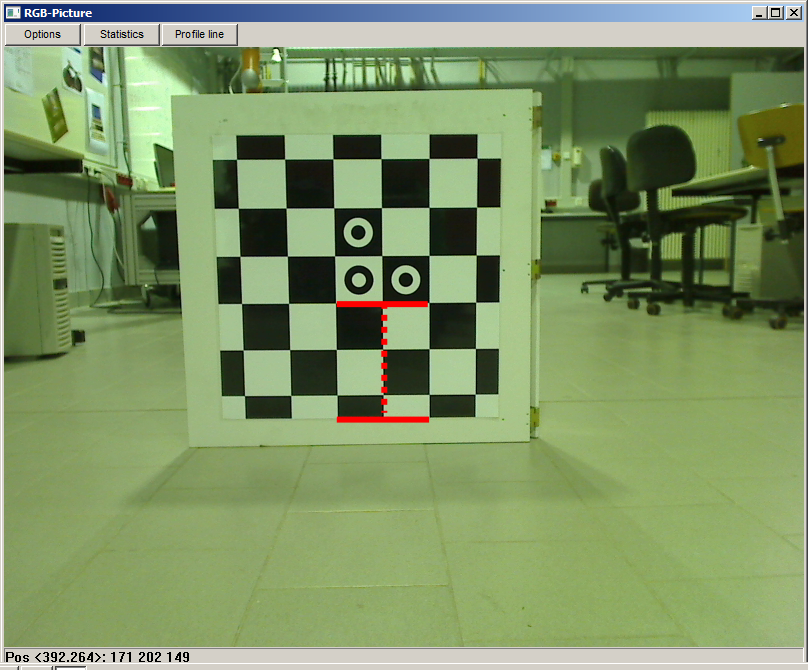
\includegraphics[width=0.55\linewidth]{bilder/camToGround_red}
    \caption{Abstand zwischen Boden und Schachbrett}
  \end{nofloat}
%TODO: bild einfügen
\item Anschließend startet man die Batchdatei \verb|calibrate.cmd| im
  Ordner \verb|\client\src\calibrate\|. Die Batchdatei fragt nun die
  Kameranummer, sowie die im vorherigen Schritt ermittelten 
 Entfernungen in mm ab und startet anschließend durch Drücken der
 Enter-Taste die Erkennung:
 \begin{nofloat}{figure}\centering
    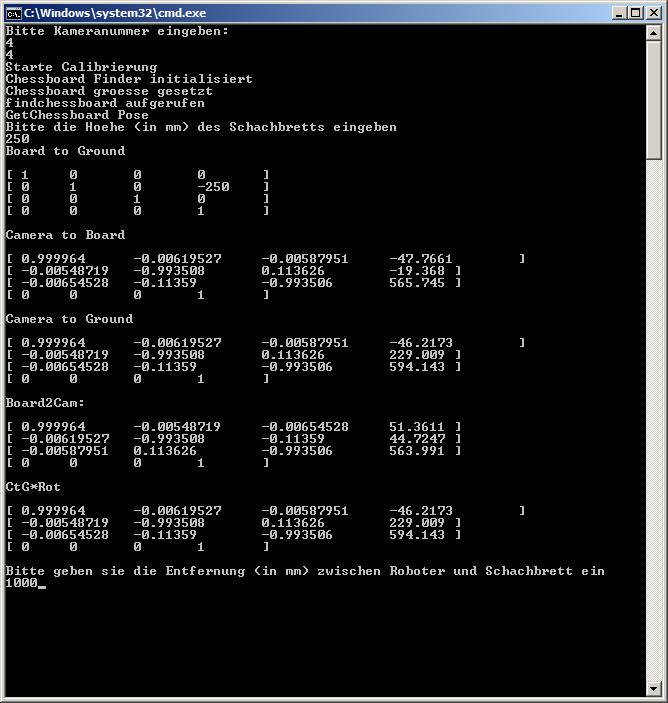
\includegraphics[width=1\linewidth]{bilder/calibrate1}
    \caption{Abfrage der zur Kalibrierung nötigen Parameter}
  \end{nofloat}\newpage
\item Die Kalibrierung ist erfolgreich, wenn folgendes Muster im
  Kamerabild angezeigt wird:
  \begin{nofloat}{figure}\centering
    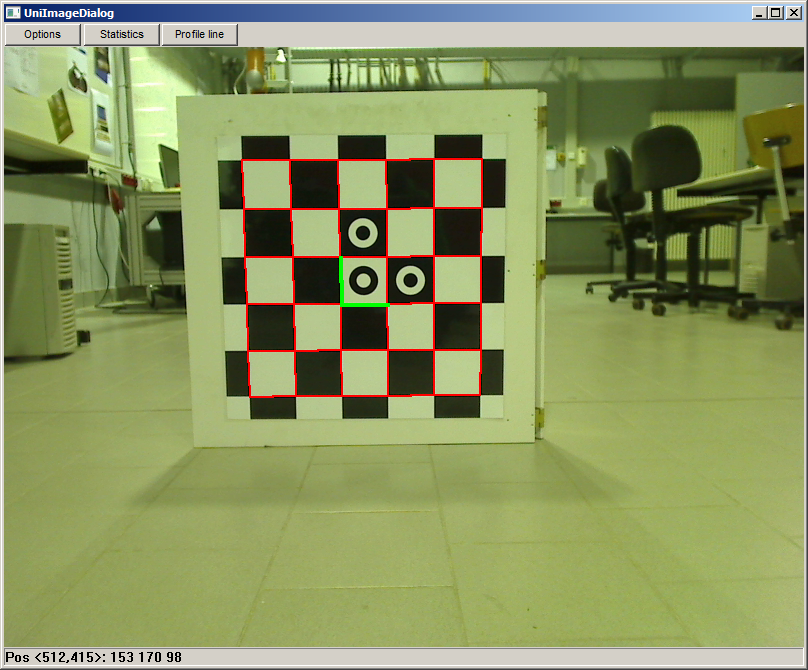
\includegraphics[width=0.7\linewidth]{bilder/calibrate2}
    \caption{Darstellung einer erfolgreichen Kalibrierung der Ballerkennung}
  \end{nofloat}
\item Dann ist im Batch-Skript die Ausführung
  des Kalibiertools mit \textless STRG \textgreater -C zu unterbrechen. Auf die Nachfrage,
  ob auch die Batchdatei unterbrochen werden soll, gibt man ,,n'' ein:
 \begin{nofloat}{figure}\centering
    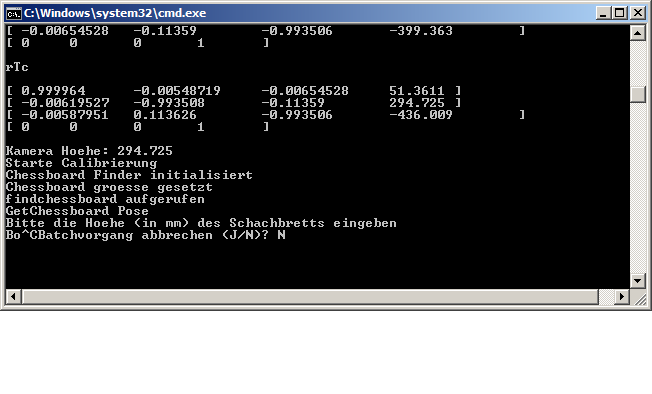
\includegraphics[width=\linewidth]{bilder/calibrate3}
  \end{nofloat}\newpage
\item Danach sollte ein neuer Ordner im aktuellen Verzeichnis mit den
  Kalibrierdaten sein. Er hat als Bezeichnung die Kameranummer
  erhalten. Im folgenden Bild sieht man das Ergebnis einer
  erfolgreichen Kalibrierung für die Kamera mit der Nummer 4, es wurde
  ein neues Verzeichnis \verb|cam4| mit den Kalibrierungsdateien erzeugt:
 \begin{nofloat}{figure}\centering
    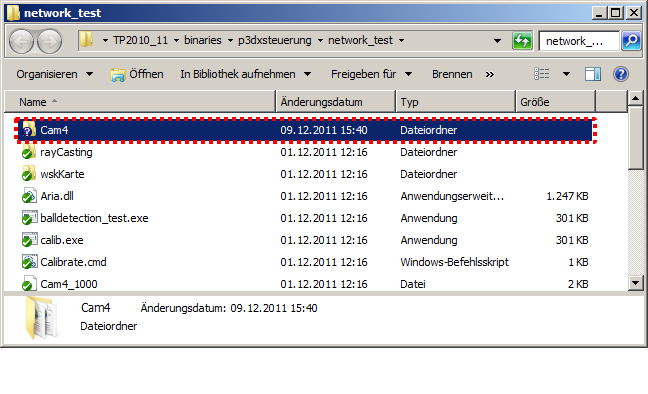
\includegraphics[width=\linewidth]{bilder/calibrate4_red}
  \end{nofloat}
\end{itemize}
%%% Local Variables: 
%%% mode: latex
%%% TeX-master: "template"
%%% End: 


\subsection{Einrichtung des Clients}%Konfiguration und Nutzung des Clients}
\label{sec:einrichtung-client}
Zunächst müssen die Webcam des Roboters und dessen serielle
Schnittstelle  mit dem Laptop, auf dem die Clientsoftware läuft,
verbunden  werden. Anschließend wird der Client über  die Datei \verb|config.cfg| eingerichtet. Eine
Erklärung und ein Beispiel finden sich im Abschnitt
\ref{sec:funktionsweise} auf Seite \pageref{aufbau_config}. Die Datei
muss sich im gleichen Verzeichnis wie die ausführbare Datei
\verb|p3dxSteuerung_threaded.exe| befinden. Ausserdem benötigt der
Client ein Batchskript zum Starten, die
Daten der Kalibrierung und Karten für die Lokalisierung. Idealerweise
erzeugt man sich für die *exe-Datei und anderen benötigten Dateien ein
eigenes Verzeichnis, wo alle benötigten Dateien rein kopiert werden.  Hierzu
empfiehlt sich der in Abbildung \ref{aufbau_laufzeit} skizzierte
Aufbau des Laufzeitverzeichnisses. Die Bedeutung der Elemente der
Verzeichnisstruktur ist der Tabelle
\ref{bedeutung_namen} zu entnehmen.
\begin{nofloat}{figure}%{l}{1\textwidth}
\label{aufbau_laufzeit}
\centering
\begin{tikzpicture}
%\tikz 
[font=\footnotesize,
       grow=right, level 1/.style={sibling distance=5em}
                   level 2/.style={sibling distance=6em}, level distance=5cm]
  \node {p3dxSteuerung} % root
     child { node {config}}
     child {node {client}
       child {node {Aria.dll}}
       child {node {calib.exe}}
       child {node {Calibrate.cmd}}
       child {node {rayCasting}
         child{node {Elevator2cm.bmp}}
         child{node {Elevator.BMP}}
         child{node {OccuMap.bmp}}
       }
       child {node {config.cfg}}
       child {node{balldetection\_test.exe}}
       child {node {p3dxSteuerung\_threaded.exe}}
       child {node {libzmq.dll}}
      % child {node {CamNo}}
       child {node {Start.bat}}
       child {node {wskKarte}
         child{node{Box.BMP}}
         child{node{Box.txt}}
         child{node {Elevator2.txt}}
         child{node {Elevator.BMP}}
         child{node {Elevator.txt}}
         }
       child {node {wtee.exe}}
   };
\end{tikzpicture}
\caption{Empfohlener Aufbau des Laufzeitverzeichnisses}  
\end{nofloat}
\begin{nofloat}{table}{
    %\begin{table}
      \centering
      \begin{tabular}{|c|p{0.8\linewidth}|}
        \hline 
        Name & Bedeutung \\ \hline
        config & Vereichnis mit den *xml-Kalibrierungsdateien\\ \hline
        client & Verzeichnis mit den Programmdateien des Clients\\ \hline
        Aria.dll, libzmq.dll & DLLs, die vom Client zur Ansteuerung
        des Roboters und zur Interprozesskommunikation benötigt werden
        \\ \hline
        %Datei der libAria, wird zur Ansteuerung des
        %Roboters benötigt\\ \hline
        calib.exe & Hilfstool zur Kalibrierung der Ballerkennung
        \footnote{Basierend auf der balldetection\_test.exe von Tobias Breuer}\\ \hline
        Calibrate.cmd &  Wrapper-Batchskript für die Kalibrierung \\ \hline
        rayCasting,  wskKarte & Verzeichnisse mit Raumkarten im
        BMP-Format\\ \hline
        config.cfg & Konfigurationsdatei für den Client\\ \hline
        balldetection\_test.exe & Miniprogramm zum Testen der
        Ballerkennung \footnote{Geschrieben von Tobias Breuer}\\ \hline
        wtree.exe & Windows-Tool, um Bildschirmausgaben von
        DOS-Programmen zu loggen und trotzdem am Bildschirm
        auszugeben.\footnote{OpenSource von Ryan Buhl unter der
          Mozilla Public License}\\ \hline
        Start.bat & Batch-Skript, um den Client auszuführen und
        gleichzeitig ein Logging mittels wtree.exe zu ermöglichen.
        %und gleichzeitigen
        %Ausgaben voder Ausgabe des Clients
        %\footnote{Dieses T
       \\ \hline
      \end{tabular}
      \caption{Die Dateien des Laufzeitverzeichnisses und ihre Bedeutung}
      \label{bedeutung_namen}
   % \end{table}
}
\end{nofloat}
%%% Local Variables: 
%%% mode: latex
%%% TeX-master: "template"
%%% End: 


\subsection{Benutzung des Clients}
\label{sec:benutz-des-clients}
Nach Konfiguration des Clients muss zunächst der Server gestartet
werden, da der Client eine funktionierende Verbindung zum Server
voraussetzt. Ist keine vorhanden, bricht er die Programmausführung ab.
Nach Start des Servers  positioniert man den Roboter in der Mitte des
Raumes, in dem die Ballsuche stattfinden soll. Anschließend schaltet
man den Roboter ein und startet den Client mit der
Stapelverarbeitungsdatei \verb|Start.bat|. Der Client startet nun und
nimm zunächst soviele Rotationen um die eigene Ache vor, wie in der
\verb|config.cfg| festgelegt worden sind. Diese dienen dazu, den
Sonar-Partikelfilter zu initialisieren, sodass der Client dann die
Position des Roboters im Raum bestimmen kann. Nach erfolgreicher
Initialisierung verbindet sich der Client mit den Server und wartet,
bis dieser die Suche startet. Sobald vom Server die Suche gestartet
wurde, wird der Client vom Server eine Liste von Punkten anfordern,
die er dann abfahren wird. Gleichzeitig öffnet sich ein Fenster, dass
das aktuelle Bild der Kamera zeigt. Es wird während der gesamten Suche
ständig aktualisiert. \\\\
Ab diesen Zeitpunkt muss man als Benutzer
nur noch den Ablauf überwachen, falls es unerwarteterweise zu
Kollisionen mit der Wand oder anderen Robotern kommt. Dies sollte zwar
aufgrund der vom Server vorgenommen Kollisionerkennung nicht
passieren, allerdings lassen sich ,,false Positives'' nicht generell
ausschließen, mehr dazu im nächsten Kapitel. Erkennt der Client
schließlich einen Ball im aktuellen Kamerabild, wird der Ball im Bild
markiert:
\begin{nofloat}{figure}\centering
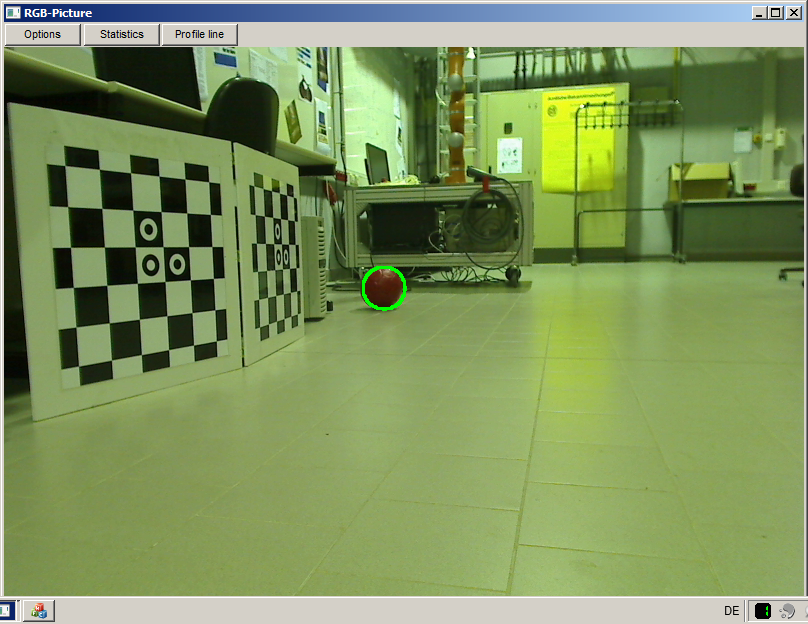
\includegraphics[width=0.75\linewidth]{bilder/balldetect}
\caption{Kamerabild bei erfolgreicher Ballerkennung}  
\end{nofloat}

Anschließend wird aus der mit den Sonar-Partikelfilter ermittelten
Position des Roboters im Raum und von der Ballerkennung zurückgebenen
Entfernung und Winkel vom Ball zum Roboter die Position des Balls im
Raum bestimmt und an den Server übermittelt. Dieser weiß nun, dass die
Ballsuche erfolgreich beendet ist und schickt allen verbundenen
Clients eine Aufforderung die Suche zu beenden. In der Folge stoppen
die Clients die Suche.
%Zunächst 
%%% Local Variables: 
%%% mode: latex
%%% TeX-master: "template"
%%% End: 
